\documentclass{cmspaper}
\usepackage{booktabs}
\usepackage{graphicx}
\usepackage{rotating}

\begin{document}

\def \mrad      {{\rm \, mrad}}
\newcommand {\cm}         {\rm   cm}
\newcommand {\mm}         {\rm   mm}
\newcommand {\m}          {\rm   m}
\newcommand {\DM}         {\Delta {\mathrm M}}
%\newcommand {\Tot}           {\mathrm{T}}
%\newcommand {\tot}     {\mathrm{t}}
\newcommand {\Xo}         {{\mathrm{X}_0}}
\newcommand {\TX}         {{\mathrm{T}_0}}
\newcommand {\tX}         {{\mathrm{t}_0}}
\newcommand {\lI}         {{\lambda_\mathrm{I}}}
\newcommand {\TI}         {{\mathrm{T}_\mathrm{I}}}
\newcommand {\tI}         {{\mathrm{t}_\mathrm{I}}}
%\newcommand {\kvect}      {{\overrightarrow{k}}}
\newcommand {\kvect}      {{\vec{k}}}

\renewcommand{\labelenumi}{\alph{enumi})}
\newcommand{\fixme}{{\bf FIXME~}}




%==============================================================================
% title page for few authors

\begin{titlepage}

% select one of the following and type in the proper number:
%   \cmsnote{2005/000}
  \internalnote{2010/000}
%  \conferencereport{2005/000}
   \date{1 Brumaio 2010}

  \title{Tracker Inner Barrel and Inner Discs\\
  Geometry and Material Budget}

  \begin{Authlist}
    Ernesto Migliore
     \Instfoot{to}{INFN Torino}
    Giacomo Sguazzoni
     \Instfoot{fi}{INFN Firenze}
  \end{Authlist}

 
  \begin{abstract}
A method to study the systematic uncertainties related to the Tracker Material Budget simulation has been developed.
The method can be applied whenever the effect of a know variation of a material budget component has to be studied.
A set of realistic material alterations to be used by physic analysis groups is proposed.
  \end{abstract} 

\end{titlepage}

\setcounter{page}{2}%JPP

\section{Introduction}

The present geometry contains the state-of-the-art of the Tracker material budget description. However there are knows issues:
\begin{description}
\item residual discrepancies between simulated and measured masses or $\DM$'s; 
\item unavoidable approximations with respect to the actual of the geometry of the physical volumes and of the material distribution and composition.
\end{description}

How to estimate the uncertainty related to these discrepancies and approximations?

The most quantitative bases of any possible way to answer are the mass discrepancies $\DM$, when available. Nevertheless, the impact of $\DM$ on the total thickness in terms of number of radiation lengths, $\TX$, or in terms of number of interaction lengths, $\TI$, does depend on how the $\DM$ is distributed among the various tracker components/materials. Once this dependence is known, it can be fed not only with $\DM$'s, but also with any other input we may consider useful to understand downstream effects on $\TX$ or $\TI$.

\section{The method}


As sketched in Fig.~\ref{fig:can}, the total thickness in terms of radiation lengths, $\TX$, has the following dependance on the $N$ materials:
\begin{equation}
\TX = \sum^N_i \rho_i \frac{\ell_i}{\Xo_i} \equiv \sum_i \tX_i.
\end{equation}
Similarly the total thickness in terms of radiation lengths, $\TI$, is
\begin{equation}
\TI = \sum^N_i \rho_i \frac{\ell_i}{\lI_i} \equiv \sum_i \tI_i.
\end{equation}
In the above relations, $i$ is the index running on the materials, $\rho$ the density, $\ell_i$ the thickness of the material $i$ and $\Xo$ and $\lI$ the radiation length and the interaction length, respectively, in $\mathrm{g}/\mathrm{cm}^2$. 

\begin{figure}[h]
\begin{center}
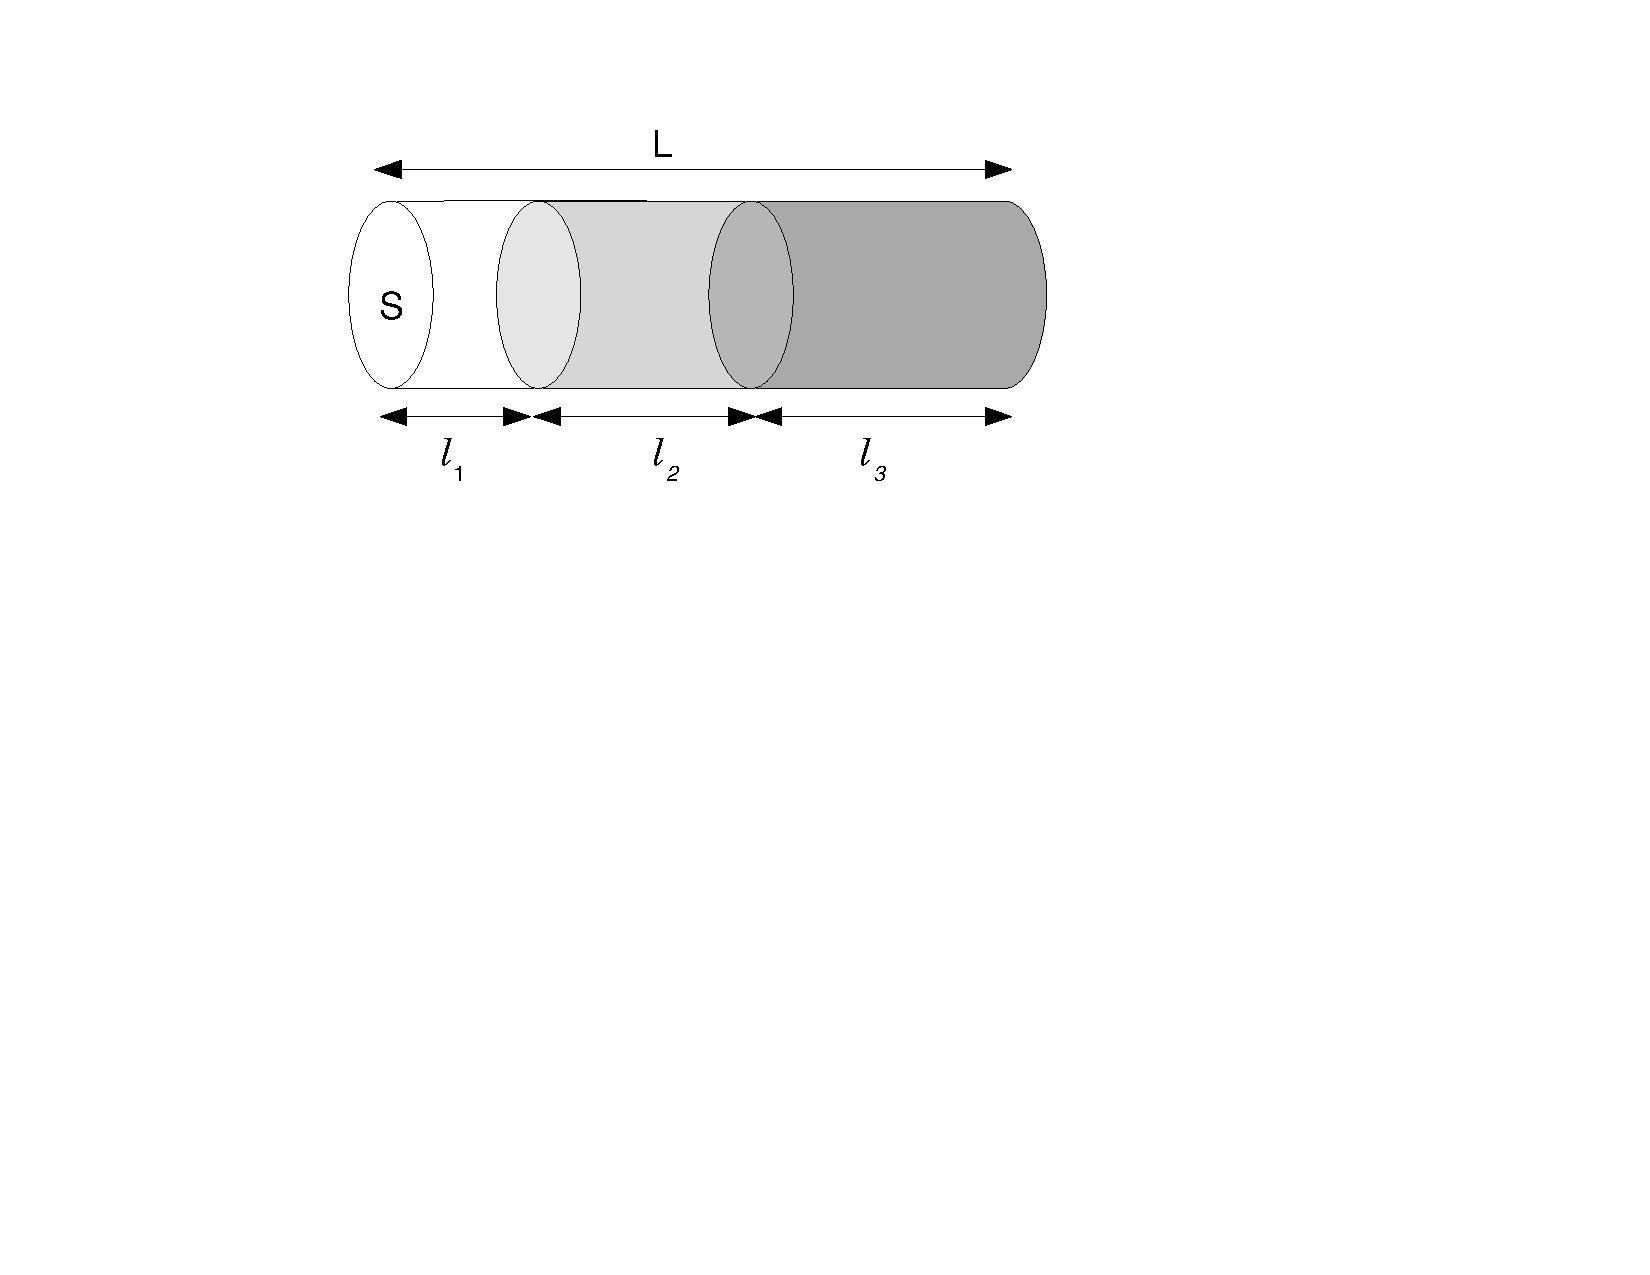
\includegraphics[width=0.5\textwidth]{fig/can.pdf}
\end{center}
\caption{Sketch of a simplified cylindrical volume made up of three different materials.}
\label{fig:can}
\end{figure}

The proposed method consists in changing in an appropriate and controlled way the material components by using a set of k-factors $\kvect\equiv(k_1, ..., k_i, ..., k_N)$ and then study the effects on $\TX$ and $\TI$. In particular
\begin{equation}
\TX = \sum^N_i \rho_i \frac{\ell_i}{\Xo_i} \rightarrow  \TX_\kvect = \sum^N_i k_i \rho_i \frac{\ell_i}{\Xo_i},
\end{equation}
and
\begin{equation}
\TI = \sum^N_i \rho_i \frac{\ell_i}{\lI_i} \rightarrow  \TI_\kvect = \sum^N_i k_i \rho_i \frac{\ell_i}{\lI_i}.
\end{equation}

\end{document}

% LocalWords:  TODO
